% !TEX root = main.tex
%%%%%%%%%%%%%%%%%%%%%%%%%%%%%%%%%%%%%%%%%%%%%%%%%%%%%%
\section{制御理論}

\subsection{本研究で用いる理論}
 本研究では,P制御,PD制御,B-dot制御則,クロスプロダクト則を検証する.

 本研究で用いる制御モデルは,電流$I$を入力とし,出力は角速度$\omega$である.
この二つの関係を運動方程式で表すと,模型の地面に平行に伸びる軸についての慣性モーメントを$J$として,

\begin{equation}
    \begin{aligned}
        J\dot{\omega} &= \boldsymbol{M \times B}\\
                       &= MB\sin\theta\\
                       &= \mu nISB\sin\theta
    \end{aligned}
\end{equation}

となり,出力の2階微分が入力$I$と出力$\theta$の正弦の積に比例しているため,非線形システムである.
また,検証の際には初期角度を90 deg とするため,$\sin \theta\approx\theta$とする近似は適切でない.
これらのことから,伝達関数を求めることが難しく,部分的モデルマッチング法のような,伝達関数を用いるゲイン決定法が使えない.
そのためP,PD制御では,制御対象のモデリングを必要としない,
限界感度法を用いてゲインの調整を行った.



%%%%%%%%%%%%%%%%%%%%%%%%%%%%%%%%%%%%%%%%%%%%%%%%%%%%%%
\subsection{P制御}
%%%%%%%%%%%%%%%%%%%%%%%%%%%%%%%%%%%%%%%%%%%%%%%%%%%%%%

 P制御では,制御量$\omega(t)$と目標値$\omega^{ref}(t)$の差を偏差$e(t)$として,コントローラを
\begin{equation}
    u(s) = k_Pe(s)
\end{equation}
で定める.
このPコントローラは一般に,ステップ状に変化する目標値や外乱に対して定常偏差が残る.
比例ゲイン$k_P$を大きくすれば,定常偏差が小さくなり,速応性が向上するが,オーバーシュートが大きくなる.
つまり,比例ゲイン$k_P$によって調整できるのは速応性と安定度のどちらか一方である.
また,多くの場合入力の大きさ$|u(t)|$には上限があるため,それに伴って$k_P$の大きさも上限がある\cite{kawata}.


%%%%%%%%%%%%%%%%%%%%%%%%%%%%%%%%%%%%%%%%%%%%%%%%%%%%%%
\subsection{PD制御}
%%%%%%%%%%%%%%%%%%%%%%%%%%%%%%%%%%%%%%%%%%%%%%%%%%%%%%

 PD制御では,制御量$\omega(t)$と目標値$\omega^{ref}(t)$の差を偏差$e(t)$として,コントローラを
\begin{equation}
    u(s) = (k_P+k_Ds)e(s)
\end{equation}
で定める.
PD制御は,粘性を高めることに相当する効果があり,P制御で問題となった振動を改善することができる.
パラメータが比例ゲイン$k_P$と微分ゲイン$k_D$の2つを持つため,速応性,安定度の両方を調整できる\cite{kawata}. 

%%%%%%%%%%%%%%%%%%%%%%%%%%%%%%%%%%%%%%%%%%%%%%%%%%%%%%
\subsection{B-dot制御則}
%%%%%%%%%%%%%%%%%%%%%%%%%%%%%%%%%%%%%%%%%%%%%%%%%%%%%%
 B-dot制御則とは,人工衛星のある1軸を規定し,その軸に沿った磁場の変化率の符号と反対の磁気モーメントを発生させる制御である.
衛星の回転運動のエネルギーを消散させることを目的とするため,角速度が0になることを目標として制御する\cite{bdot}.

 静止状態において,地磁気ベクトル$\boldsymbol{B}_\mathrm{geo}$が,衛星を基準とする$x-y$平面上のx軸に沿っているとする.
t秒後の地磁気の$x$成分$B_x$,$y$成分$B_y$は,地磁気ベクトルの大きさ$B_o=|\boldsymbol{B}_\mathrm{geo}|$,角速度$\omega_z$を用いて,

\begin{align}
    \left\{
        \begin{aligned}
            B_x &= B_o\cos\omega_zt\\
            B_y &= -B_o\sin\omega_zt\\
        \end{aligned}                    
    \right.
\end{align}

で表される.図を用いて表すと,図\ref{fig:geo}のようになる.

\begin{figure}[H]
	\centering
		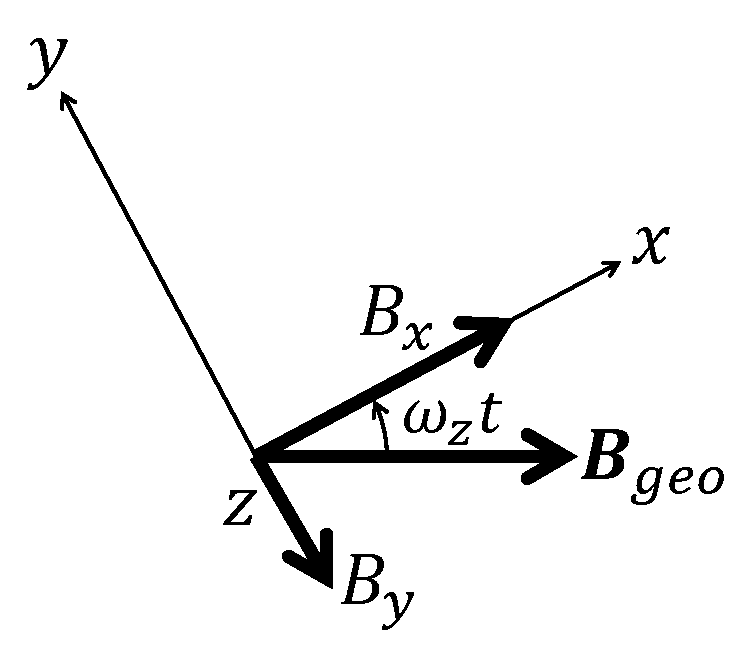
\includegraphics[scale=0.5]{./figure/B-dot1-crop.pdf}
		\caption{地磁気ベクトルの表現}
		\label{fig:geo}
\end{figure}

 そして,それぞれの時間変化は,

\begin{align}
    \left\{
        \begin{aligned}
            \dot{B_x} &= -B_o\omega_z\sin\omega_zt = B_y\omega_z\\
            \dot{B_y} &= -B_o\omega_z\cos\omega_zt = -B_x\omega_z
        \end{aligned}                    
    \right.
\end{align}

である.
初期位相および目標角を0 [deg],$k$を正の定数とすると,目標磁気モーメントは,

\begin{equation}
    M_x = -k\dot{B_x} = -B_o\omega_z\sin\omega_zt
\end{equation}

で決定される.
このとき,生じるトルクは,
\begin{equation}
    \begin{aligned}
        \mathrm{T_z} &= M_x \times B_y\\
                     &= (kB_o\omega_z\sin\omega_zt)(-B_o\sin\omega_zt)\\
                     &= -kB_o^2\omega_z\sin^2\omega_zt
    \end{aligned}
\end{equation}

である.
衛星の1回転にわたり,$\sin^2 \omega_zt$の絶対値の平均値は0.5となるため,その平均値は

\begin{equation}
    \mathrm{T_\mathrm{z,ave}} = \frac{-kB_o^2\omega_z}{2}
\end{equation}

で表される.このトルクから,衛星の回転運動についての運動方程式は,

\begin{equation}
    J_z\dot{\omega_z} = \mathrm{T_\mathrm{z,ave}} = \frac{-kB_o^2\omega_z}{2}
\end{equation}

となる.これを変形して,

\begin{equation}
    \dot{\omega_z}+\frac{kB_o^2}{2J_z}\omega_z = 0
\end{equation}

が得られる.この微分方程式は,$\tau=\frac{J_z}{kB_o^2}$とすると,衛星の初期角速度を$\omega_{z_o}$として,

\begin{equation}
    \omega_z = \omega_{z_o}e^{-\frac{t}{2\tau}} 
\end{equation}

となり,指数関数的に角速度が減少することがわかる.本研究では,$z$軸について磁気トルカを1つ用いて制御を行う.\\
 次に,磁気トルカを1つ増やし,それを$y$軸に添わせることを考える.
目標磁気モーメントは

\begin{equation}
    M_y = -k\dot{B_y} = kB_o\omega_z\cos\omega_zt
\end{equation}

となる.
2つの磁気トルカにより生じるトルクを合成すると,

\begin{equation}
    \begin{aligned}
        T_z &= M_xB_y - M_yB_x\\
            &= (kB_o\omega_z\sin\omega_zt)(-B_o\sin\omega_zt)-(kB_o\omega_z\cos\omega_zt)(B_o\cos\omega_zt)\\
            &= -kB_o^2\omega_z\sin^2\omega_zt - kB_o^2\omega_z\cos^2\omega_zt\\
            &= -kB_o^2\omega_zt\\
            &= \dot{L} = J_Z\dot{\omega_z}
    \end{aligned}
\end{equation}

この微分方程式の$\omega_z$の解は,

\begin{equation}
    \omega_z = \omega_{z_o}e^{-\frac{t}{\tau}} 
\end{equation}

となるので,減衰の時定数が半分となることがわかる.


 次に,磁気トルカをもう1つ追加したときを考える.3つの磁気トルカがそれぞれ直交するように衛星に配置されているとき,
$x-y$平面,$z-x$平面,$y-z$平面について,B-dot制御を考える.
$x$軸回り,$y$軸回りの角速度を$\omega_x$,$\omega_y$とすると,

\begin{align}
    \left\{
        \begin{aligned}
            B_z &= B_o\cos\omega_yt\\
            B_x &= -B_o\sin\omega_yt\\
        \end{aligned}                    
    \right.
    ,\quad
    \left\{
        \begin{aligned}
            B_y &= B_o\cos\omega_xt\\
            B_z &= -B_o\sin\omega_xt\\
        \end{aligned}                    
    \right.
\end{align}

で表される.
そして,それぞれの時間変化は,

\begin{align}
    \left\{
        \begin{aligned}
            \dot{B_z} &= -B_o\omega_y\sin\omega_yt = B_x\omega_y\\
            \dot{B_x} &= -B_o\omega_y\cos\omega_yt = -B_z\omega_y
        \end{aligned}                    
    \right.
    ,\quad
    \left\{
        \begin{aligned}
            \dot{B_y} &= -B_o\omega_x\sin\omega_xt = B_z\omega_x\\
            \dot{B_z} &= -B_o\omega_x\cos\omega_xt = -B_y\omega_x
        \end{aligned}                    
    \right.
\end{align}

となる.(1.2)式と(1.13)式を重ね合わせると,

\begin{equation}
    \left\{
        \begin{aligned}
            \dot{B_x} = B_y\omega_z - B_z\omega_y\\
            \dot{B_y} = B_z\omega_x - B_x\omega_z\\
            \dot{B_z} = B_x\omega_y - B_y\omega_x
        \end{aligned}
    \right.
\end{equation}

となることから,$xyz$空間において,地磁気の時間変化は

\begin{equation}
    \boldsymbol{\dot{B} = B \times \omega}
\end{equation}

で表され,
目標磁気モーメントは,

\begin{equation}
    \begin{aligned}
        \boldsymbol{M} &= -k \boldsymbol{\dot{B}}\\
                       &= -k(\boldsymbol{B \times \omega})
    \end{aligned}
\end{equation}

で求められる.

\subsection{クロスプロダクト則}
 クロスプロダクト則は,衛星の姿勢情報を必要とせず,観測した地磁気ベクトルと,予測される目標姿勢での地磁気ベクトル,現在の角速度を用いて行う制御である.
PD制御との相違点は,角度情報を角度センサでなく磁気ベクトルの外積から得ているという点である.
B-dot制御則との違いは,B-dot制御則は角速度(地磁気ベクトルの時間変化)を0に指向する,簡単にいわばD制御のようなものであるのに対し,クロスプロダクト則は,姿勢を目標値に指向し,角速度情報を用いる,いわばPD制御のようなものという点である.
 衛星座標系で測定された地磁気ベクトル$\boldsymbol{b_m}$,その衛星の位置が目標姿勢を保っていた場合の地磁気ベクトル$\boldsymbol{b_r}$を用いて,
外積ベクトル$\boldsymbol{c}$を

\begin{equation}
    \boldsymbol{c} = \boldsymbol{\frac{b_m}{|b_m|}\times\frac{b_r}{|b_r|}}
\end{equation}

で定める.
これと,角速度の誤差$\Delta\omega = [\omega_x\space\omega_y\space\omega_z]$を用いて,
目標トルクが

\begin{equation}
    \boldsymbol{T}_R = K\boldsymbol{c}+k\Delta\boldsymbol{\omega}\\
\end{equation}

で定められる.なお,$K,k$は,

\begin{equation}
    K = 
    \begin{bmatrix}
        K_x & 0 & 0 \\
        0 & K_y & 0 \\
        0 & 0 & K_z \\
    \end{bmatrix}
    ,k =
    \begin{bmatrix}
        k_x & 0 & 0 \\
        0 & k_y & 0 \\
        0 & 0 & k_z \\
    \end{bmatrix}
\end{equation}

で定められる係数行列である.
本研究は$z$軸方向の一軸のみ制御する.$c_z = b_{m_x}b_{r_y} - b_{m_y}b_{r_x}$なので,

\begin{equation}
    T_{R_z} = K_x c_z + k_x \omega_z 
\end{equation}

で,
磁気トルカにより発生するトルクの式より,磁気トルカの目標磁気モーメントは,

\begin{equation}
    \begin{aligned}
        T_z = M_x B_y - M_y B_x &= M_x B_y \quad(M_y = 0)\\
         K_x c_z + k_x \omega_z &= M_x B_y\\
                            M_x &= \frac{K_x c_z + k_x \omega_z}{B_y}
    \end{aligned}
\end{equation}

で求められる\cite{cross}.